\section{校区环境}

北邮现在使用中的校区一共两个,即西土城路校区(海淀区,本部)和沙河校区(昌平区)\footnote{另有西城区小西天校区(校舍)和昌平区宏福校区(接近弃用),目前和大家关系不大,唯有实验课偶尔会去一两次}。校本部位于海淀区西土城路10号,面积很小,住宿条件相对较差,但交通便利,对面就是北师大,周围美食众多。目前,大部分大三大四的本科生及多数研究生在本部学习。沙河校区是新生入学的校区,位于昌平区沙河镇南丰路{\small{}与高教园南三街交口向北400米路东\sout{(我知道写这些你不会看的)}}。规划面积很大(大概本部三倍)但是实际建成只有一半左右,住宿学习环境好,但比较偏僻,被两个地铁站夹在中间导致出行不便。所有新生都将在沙河校区入学并在这至少读完大一。

按照学校最新的安排,各个学院的本科生从沙河搬到本部的时间有下表:

\begin{tabular}{cc}
    \toprule
    学院 & 搬迁时间(学年开始) \\
    \midrule
    计算机学院(国家示范性软件学院) & 大二 \\
    经济管理学院 & 大二 \\
    国际学院 & 大二\\
    信息与通信工程学院 & 大三 \\
    电子工程学院 & 大三 \\
    人工智能学院 & 大三 \\
    \bottomrule
\end{tabular}

网络空间安全学院、现代邮政学院(自动化学院)、理学院、人文学院、数字媒体与设计艺术学院不搬至本部(即在沙河校区读完本科四年)。

\begin{center}
    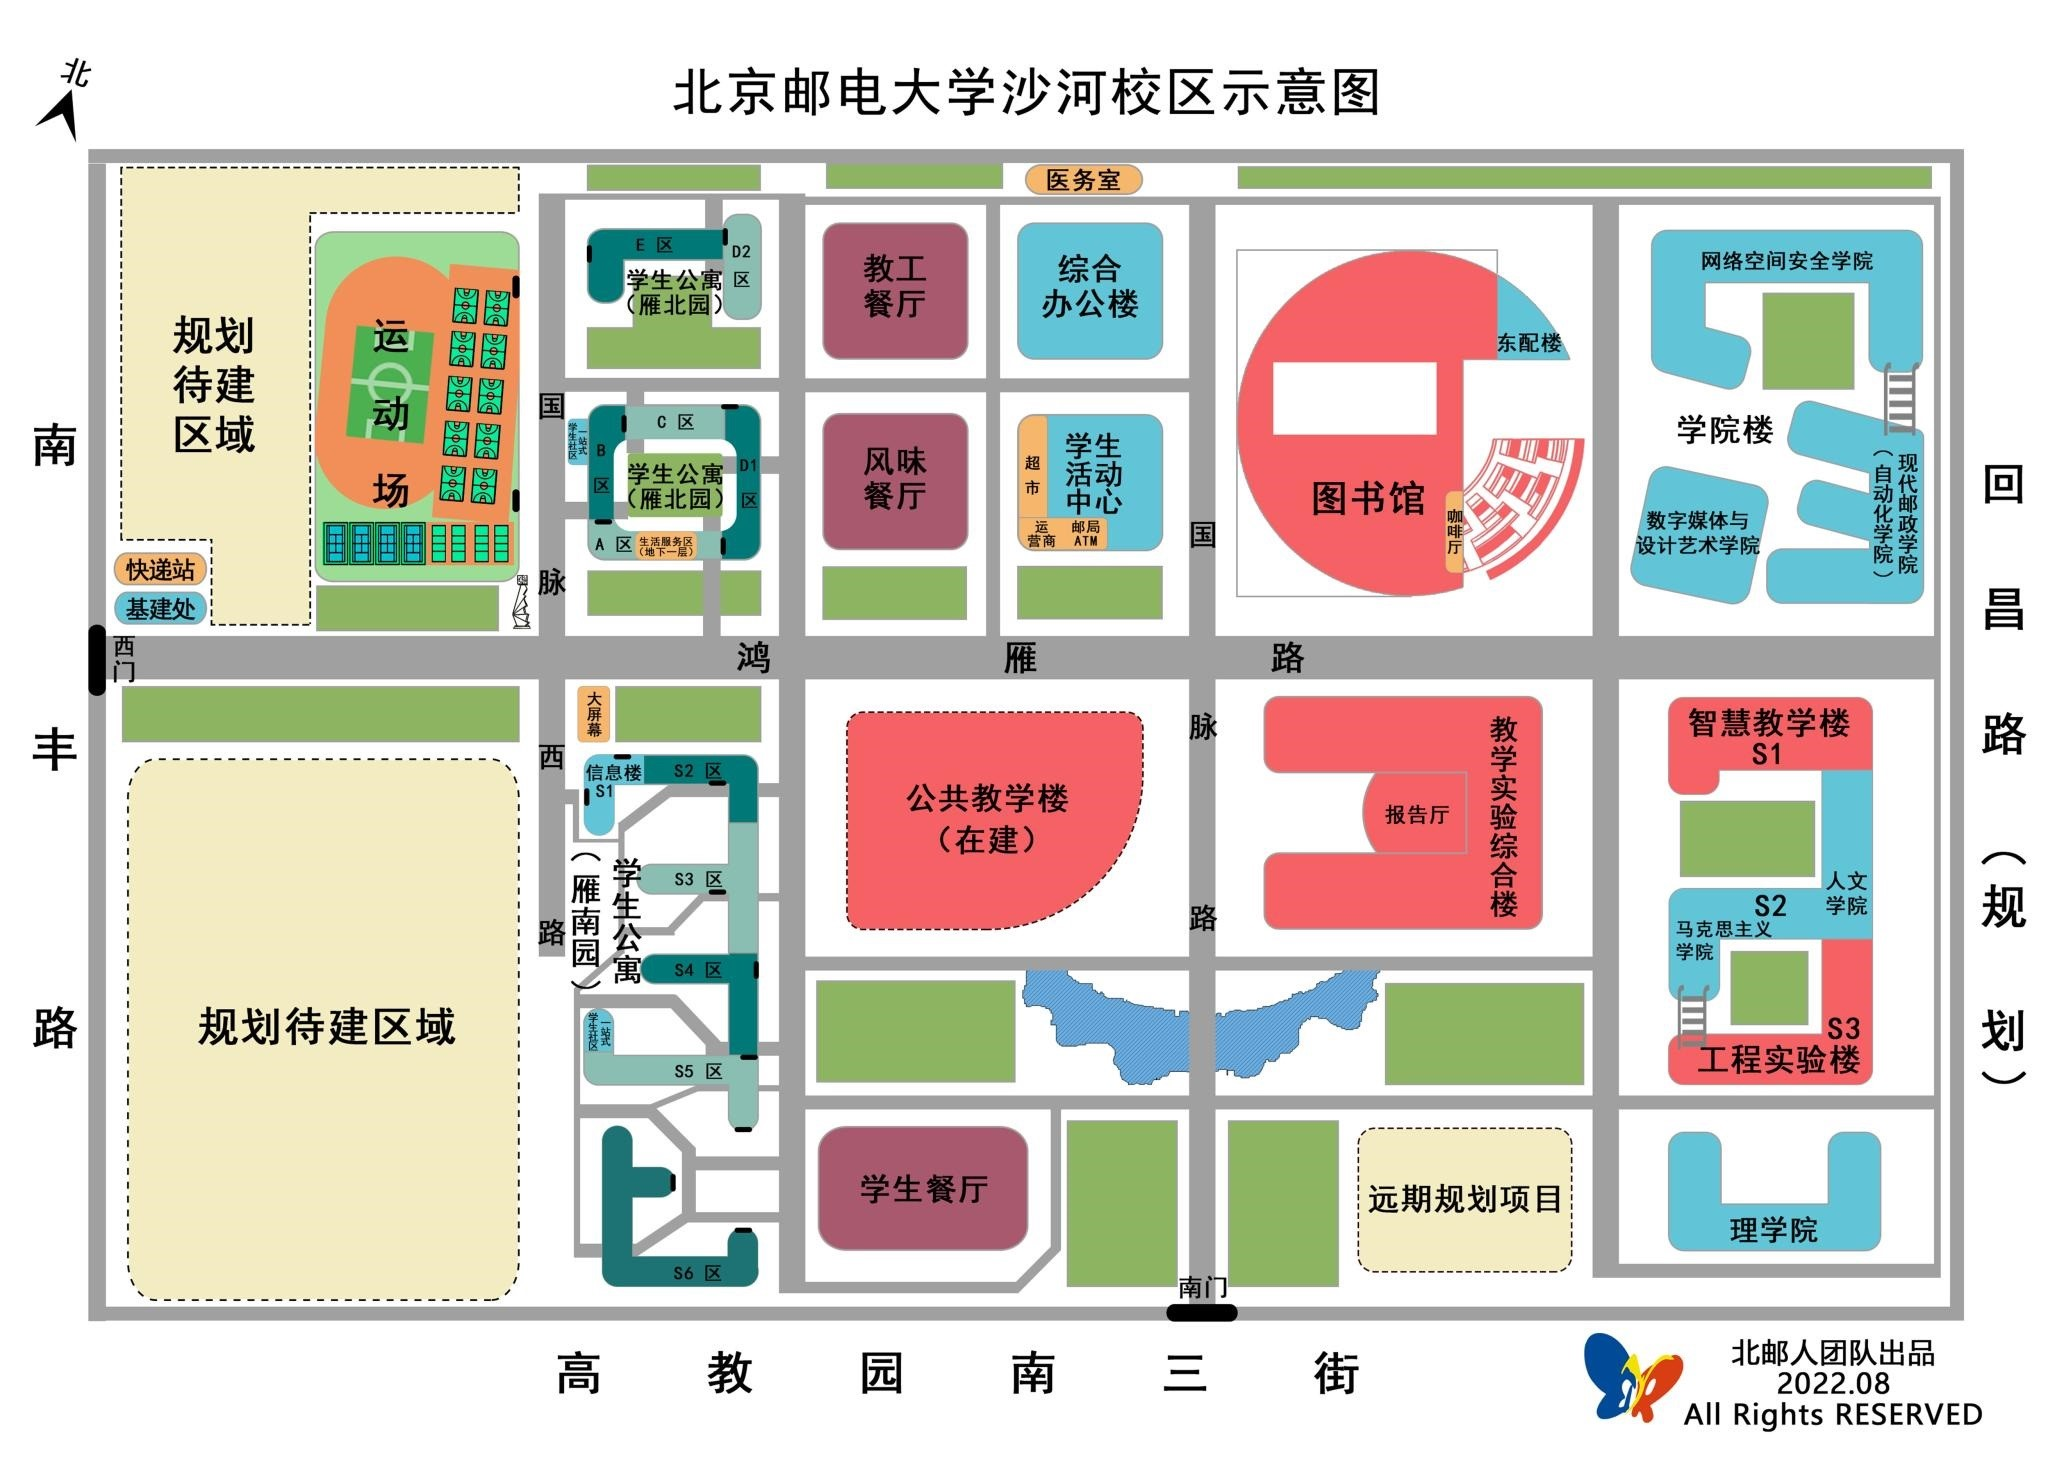
\includegraphics[width=0.80\textwidth]{images/shahe-map.jpg}
\end{center}

\faq{校园到底有多大?绕一圈要多久?}

很小,真的很小。本部绕一圈仅需10分钟,沙河大概也就20分钟(由于四周还没建设完成,所以(从物理上)根本无法绕圈(笑))。{\small (不过小也有小的好处,比如说可以7:55起床去上8:00的课)}

\faq{我什么时候会从沙河搬到本部?}

除参照上表外,学校已经在招生章程中写出了各专业的办学地点。从2022级本科生开始,大部分学院(包括计算机学院在内)的大一会在沙河校区完成,大二至大四均会在校本部就读。\footnote{可在\href{https://zsb.bupt.edu.cn/info/1005/1992.htm}{此}查看各专业办学地点}

\faq{有校车吗?免费吗?}

有,校车往返本部和沙河,并且是免费的。学期开始后可以在学校的微信企业号上查询具体班次。由于校车要优先服务老师和本部学生,所以有可能会没有位子。

正常情况下需用时35-55分钟,相较于地铁(昌平线直达或换乘)会更快一点。

沙河校区在图书馆十字路口处登车,本部在教三楼西侧登车。高峰时段可能需要提前去排队,建议提前10到15分钟到指定地点等待,否则大概率是没位置的。

\faq{寒暑假我可以住在学校吗?}

可以住在学校,但由于本科生从沙河校区搬往本部是在新学年开始时进行,所以下一学年搬往本部的同学,暑假只能住在沙河校区。

\faq{在校园里如何付钱?}

除去最常用的校园卡之外,还可以使用一款叫做“完美校园”的App,关联校园卡后可以在忘记带或者懒得带校园卡的情况下在食堂进行支付。
